% Provenance (never printed): see sources/outline_sources.md (Year 3: Gibbs
% energy and the phase rule in rocks, chemical potential recalled from the
% chemistry book; ternary diagrams; pseudosections, principle). Brief:
% sources/book5/BRIEFS.md, ch. 11. Curves from figdata/bachelor-3/
% gasp_tables.py, schreinemakers.py and regular_solution.py. Exercise and
% problem values in the Book 5 scratch calculator calc/ch11.py.
\chapter{الديناميكا الحرارية للصخور}\label{ch:b3:petrological-thermodynamics}

نما بلّورُ الجارنيت، الذي يبلغ قطره بضعة مليمترات، منطقةً تلو أخرى أثناء دفن الشيست الذي يحويه وتسخينه.
ولا يزال حافّه يسجّل، في محتواه من الكالسيوم والحديد والمغنيسيوم،
آخرَ توازنٍ بلغه مع البيوتايت والبلاجيوكلاز المحيطَين به.
حوّل مجلد السنة الثانية مثل هذه التراكيب إلى درجة حرارة وضغط
بمعادلتين معايَرتين. يفتح هذا الفصل الصندوق: من أين تأتي المعادلتان،
وإلى أيّ حدّ يمكن الوثوق بجداول الإنثالبيات والإنتروبيات المقيسة،
وكم عدد المعادن التي يمكن أن يحويها الصخر، وكيف تمتزج المحاليل الصلبة وتنفصل،
وكيف يحوّل الحاسوب التركيب الكلي إلى خريطة للتجمّعات
المعدنية التي ينبغي أن يُبيّنها.

\begin{recall}
طاقة جيبس والجهد الكيميائي والنشاط وثابت التوازن
والتباين وقاعدة الأطوار وفجوة الامتزاج وقاعدة الرافعة
موجودة في المجلدات الجامعية لكتب الكيمياء. أمّا التفاعل أحادي التغيّر،
وميل كلابيرون $\Delta_rS/\Delta_rV$، ونقطة اللاتغيّر، ومخطط الألومينوسيليكات
المحسوب من الجداول، فهي في مجلد السنة الثانية، في فصله عن السحنات المتحوّلة؛
والمحرار الجيولوجي ومقياس الضغط الجيولوجي، ومحرار التبادل بين الجارنيت والبيوتايت،
ومقياس الضغط GASP، في فصله عن مسارات P--T--t؛
والمخططات ثلاثية المكوّنات والمنحنى المشترك للتبلّر، في فصله عن الصهارات. ويرد
المحلول الصلب وأطرافه النقية في مجلد السنة الأولى، في فصله عن
المعادن.
\end{recall}

\section{التوازن انطلاقًا من الجداول}\label{sec:b3:petrological-thermodynamics:tables}

في تفاعلٍ بين معادن ذات تركيب ثابت، يتحقّق التوازن عند درجة الحرارة
$T$ والضغط $P$ حين يكون $\Delta_rG(T, P) = 0$. وتعطي الجداول، عند
\qty{298.15}{K} و\qty{1}{bar}، إنثالبيَّ التكوين والإنتروبيَ والحجمَ المولي لكلّ معدن،
والسعةَ الحرارية $C_p(T)$ عند درجات الحرارة الأعلى. وقد أخذ مجلد السنة الثانية
$\Delta_rH$ و$\Delta_rS$ و$\Delta_rV$ ثوابتَ. وتتمثّل
النتيجة العامة فيما يلي.

\begin{theorem}[طاقة جيبس للتفاعل عند $T$ و$P$]\label{thm:b3:petrological-thermodynamics:dg}
ليكن للتفاعل، عند $T_0 = \qty{298.15}{K}$ و\qty{1}{bar}،
الإنثالبي $\Delta_rH^\circ$ والإنتروبي $\Delta_rS^\circ$، وتغيّرُ السعة الحرارية
$\Delta_rC_p(T)$، وبين المواد الصلبة تغيّرَ الحجم $\Delta_rV$
مستقلًّا عن $T$ و$P$. عندئذٍ
\[
  \Delta_rG(T, P) = \Delta_rH^\circ + \int_{T_0}^{T}\Delta_rC_p\,\mathrm dT
  - T\Bigl(\Delta_rS^\circ + \int_{T_0}^{T}\frac{\Delta_rC_p}{T}\,\mathrm dT\Bigr)
  + (P - 1)\,\Delta_rV ,
\]
وخطّ التوازن هو $P = 1 - \Delta_rG(T, 1)/\Delta_rV$.
\end{theorem}

\begin{proof}
عند \qty{1}{bar}، $(\partial\Delta_rH/\partial T)_P = \Delta_rC_p$
و$(\partial\Delta_rS/\partial T)_P = \Delta_rC_p/T$؛ وبالتكامل من $T_0$
ينتج $\Delta_rH(T)$ و$\Delta_rS(T)$، ومنه $\Delta_rG = \Delta_rH -
T\Delta_rS$. وعند $T$ ثابتة، $(\partial\Delta_rG/\partial P)_T = \Delta_rV$،
ثابتةٌ بالفرض؛ وبالتكامل من 1 إلى $P$ يُضاف $(P - 1)\Delta_rV$.
وبوضع $\Delta_rG(T, P) = 0$ نحصل على الخط.
\end{proof}

يتلاشى التكاملان جزئيًّا: مجموعهما هو $\int_{T_0}^T\Delta_rC_p(1 -
T/T')\,\mathrm dT'$، ويكون العامل $1 - T/T'$ سالبًا وصغيرًا
عندما يكون $T'$ قريبًا من $T$. وبين المواد الصلبة يكون $\Delta_rC_p$ نفسه صغيرًا،
لأنّ السعة الحرارية للمعدن تقارب مجموع سعات أكاسيده
المكوّنة له. لذلك يكون تقريبُ الخواصّ الثابتةِ جيّدًا، وتبيّن الجداولُ
مدى جودته. وبالنسبة إلى تفاعل GASP،
\[
  \ce{3 CaAl2Si2O8 <=> Ca3Al2Si3O12 + 2 Al2SiO5 + SiO2},
\]
يعطي الجدول الملخّص $\Delta_rH^\circ = \qty{-36.3}{kJ}$،
$\Delta_rS^\circ = \qty{-130.7}{J.K^{-1}}$ و$\Delta_rV =
\qty{-6.61}{J.bar^{-1}}$، فيكون خطّ الميل \qty{19.8}{bar/K}؛ أمّا
الجداول عالية الحرارة، التي تتضمّن السعات الحرارية، فتعطي
$\Delta_rG$ عند كلّ \qty{100}{K}، ويختلف الخطّان بأقلّ من
\qty{0.12}{kbar} حتى \qty{1200}{K} (انظر الشكل أدناه).
% ledger: rh95:gasp-298, rh95:gasp-ht

ولا تتّفق التجارب بالقدر نفسه. وحين يُعكس التفاعل في مكبس الأسطوانة-المكبس عند
900 إلى \qty{1250}{\celsius}، يقع التفاعل أعلى من الجداول بمقدار \qty{0.9}{kbar}
عند \qty{627}{\celsius}، وبمقدار \qty{1.9}{kbar} أعلى عند
\qty{927}{\celsius}. ومع $\Delta_rV = \qty{-6.61}{J.bar^{-1}}$،
\qty{1.9}{kbar} يمثّل خطأً مقداره \qty{12.6}{kJ} في $\Delta_rH$؛ أمّا
عدم اليقين في إنثالبيّات التكوين الأربع: \qty{3.2}{kJ} للغروسولار،
و\qty{2.0}{kJ} للأنورثيت والكيانيت، و\qty{1.0}{kJ} للكوارتز،
تتراكم لتبلغ نحو \qty{8}{kJ} في $\Delta_rH$. وتحدّد القياسات الحرارية كلّ معدن
إلى بضعة كيلوجولات؛ ويضاعف تفاعلٌ بين وحدات صيغ كبيرة
هذه الأخطاء ثم يقسمها على تغيّر حجمٍ صغير.
% ledger: rh95:gasp-298, kn88:gasp

\begin{definition}[مجموعة البيانات الديناميكية الحرارية المتّسقة داخليًّا]\label{def:b3:petrological-thermodynamics:dataset}
\emph{مجموعة البيانات الديناميكية الحرارية المتّسقة داخليًّا}\index{مجموعة البيانات الديناميكية الحرارية المتّسقة داخليًّا} هي
جدول للخواص القياسية لعدد كبير من المعادن والموائع
(إنثالبي التكوين والإنتروبي والحجم والسعة الحرارية
والتمدّد الحراري والانضغاطية) مُعدَّلةً معًا ضمن
حدود عدم اليقين في القياسات الحرارية، بحيث يمرّ كلّ توازن يُحسب منها
بالتجارب المعكوسة التي ضُبطت عليها.
\end{definition}

تُضبط مجموعة كهذه مرّةً واحدة، بطريقة المربعات الصغرى الموزونة أو البرمجة الخطّية
على جميع القيود معًا، ثم تُستخدم في كلّ
تفاعل بين معادنها، بما فيها التفاعلات التي لم تُدرس قطّ في
المختبر. وأرقامها ليست قياسات مستقلّة: فقد تُزاح إنثالبيّةٌ واحدة
بمقدار كيلوجول لتلائم تفاعلًا تشترك فيه. والقيم المأخوذة
من مجموعات بيانات مختلفة لا يجوز خلطها أبدًا.

\begin{omfigure}
\begin{tikzpicture}
\begin{axis}[omrecord, width=0.78\linewidth, height=0.5\linewidth,
  xlabel={درجة الحرارة \babelsublr{(\unit{\celsius})}}, ylabel={الضغط \babelsublr{(\unit{kbar})}},
  xmin=400, xmax=1300, ymin=0, ymax=30, legend style={font=\scriptsize,
  at={(0.03,0.97)}, anchor=north west, legend cell align=left}]
% computed in figdata/bachelor-3/gasp_tables.py
\fill[omLithLime!60] (axis cs:900,19) rectangle (axis cs:1250,28);
\addplot[red!70!black, very thick] table[x=tc, y=p_kn88] {figdata/out/bachelor-3-gasp_tables-lines.dat};
\addlegendentry{\foreignlanguage{arabic}{التجربة (الأطراف النقية)}}
\addplot[omDef, thick, densely dashed] table[x=tc, y=p_const] {figdata/out/bachelor-3-gasp_tables-lines.dat};
\addlegendentry{\foreignlanguage{arabic}{الجداول مع ثبات $\Delta_rH$ و$\Delta_rS$}}
\addplot[omDef, only marks, mark=*, mark size=1.8pt] table[x=tc, y=p_table] {figdata/out/bachelor-3-gasp_tables-tables.dat};
\addlegendentry{الجداول مع السعات الحرارية}
\node[font=\scriptsize, align=center] at (axis cs:1075,26.3) {التجارب\\المعكوسة};
\node[font=\scriptsize] at (axis cs:560,4) {الأنورثيت};
\node[font=\scriptsize, align=center] at (axis cs:560,17) {الغروسولار + الكيانيت\\+ الكوارتز};
\end{axis}
\end{tikzpicture}

\par\smallskip{\small تفاعل GASP للأطراف النقية، 3 الأنورثيت = الغروسولار +
2 الكيانيت + الكوارتز، محسوبًا من جداول القياس الحراري بخصائص ثابتة
(بخط متقطّع) وبالسعات الحرارية (بنقاط)، والخطّ المُلاءَم
للتجارب المعكوسة المُجراة في المدى المظلَّل (الأحمر، مُستقرَأ إلى ما دون
\qty{900}{\celsius}).}\label{fig:b3:petrological-thermodynamics:gasp}
\end{omfigure}
% ledger: rh95:gasp-298, rh95:gasp-ht, kn88:gasp

\section{قاعدة الأطوار في الصخور}\label{sec:b3:petrological-thermodynamics:phase-rule}

تعطي قاعدة الأطوار في الكيمياء التباين $F = c - p + 2$ لنظام من
$c$ مكوّنات في $p$ طورًا. الصخر نظام كهذا، وتُبيّن معادنه
أيَّ جزءٍ من مستوى الضغط--درجة الحرارة بلغ فيه التوازن.

\begin{proposition}[قاعدة الأطوار المعدنية]\label{prop:b3:petrological-thermodynamics:goldschmidt}
صخرٌ بلغ التوازن عند ضغط ودرجة حرارة يُختاران
بحريّة ضمن منطقة من مستوى الضغط--درجة الحرارة، يحتوي على عدد من الأطوار
لا يزيد على عدد مكوّناته: $p \le c$. وهذه هي
\emph{قاعدة الأطوار المعدنية}\index{قاعدة الأطوار المعدنية}.
\end{proposition}

\begin{proof}
تعطي قاعدة الأطوار $F = c - p + 2$ متغيّرات شدّية مستقلّة. فإذا أمكن
تغيير الضغط ودرجة الحرارة معًا دون تغيّر التجمّع، فإنّ اثنين منها حرّان:
$F \ge 2$، ومنه $p \le c$. والصخر ذو $p = c + 1$ طورًا يقع
على خط أحادي التغيّر؛ ومع $p = c + 2$ عند نقطة لا متغيّرة؛ وكلاهما
غير مرجَّح لصخر يُؤخذ عشوائيًّا.
\end{proof}

الصخر الذي يخرق القاعدة إمّا أنّه بلغ التوازن على خط تفاعل، وقد تُظهره
أنسجتُه، أو أنّه لم يبلغ التوازن في مجموعه قطّ: كالأنسجة الهالية،
والمعادن المتطبّقة والحبيبات المتبقّية أسباب شائعة. ويحتاج عدّ المكوّنات
إلى عناية. المكوّن الموجود في طور واحد ذي تركيب ثابت، مثل
الزركون، يمكن إسقاطه مع طوره؛ والمكوّن المثبَّت بخزّان خارجي،
مثل الماء عندما يتدفّق سائل عبر الصخر، لا يُحسب
حرًّا، لأنّ جهده الكيميائي مفروض.

حول نقطة لا متغيّرة لا تتقاطع الخطوط أحادية التغيّر عشوائيًّا. في نظام
من $c$ مكوّنات، يلتقي عند النقطة $c + 2$ طورًا، وتنبثق منها $c + 2$
تفاعلًا، يُكتب كلٌّ منها بين $c + 1$ طورًا ويُسمّى باسم
الطور الذي يُغفله، بين قوسين.

\begin{definition}[تحليل شراينماكرز]\label{def:b3:petrological-thermodynamics:schreinemakers}
\emph{تحليل شراينماكرز}\index{تحليل شراينماكرز} هو الأسلوب
الذي يرتّب الخطوط أحادية التغيّر حول نقطة لا متغيّرة انطلاقًا من
تراكيب الأطوار وحدها، قبل أيّ قياس لخصائصها
الديناميكية الحرارية: فيحدّد ترتيب الخطوط، وجانب كلٍّ منها
المستقرّ، وتجمّعات كلّ قطاع بينها.
\end{definition}

\begin{method}[قواعد شراينماكرز]\label{met:b3:petrological-thermodynamics:schreinemakers}
(1) اكتب $c + 2$ تفاعلًا، كلٌّ منها يُغفل طورًا واحدًا. (2) كلّ خطّ
مستقرّ على جانب من النقطة وشبه مستقرّ على الجانب الآخر. (3)
الامتداد شبه المستقرّ للخطّ ($i$)، الذي يُغفل الطور $i$، يقع في قطاع
يكون فيه $i$ مستقرًّا. (4) لا يزيد أيّ قطاع بين خطّين مستقرّين متتاليين
على \ang{180}. (5) عبر الخطّ، تكون التجمّعات على جانبيه
هي تجمّعات طرفي تفاعله. وتثبيت خطّ واحد بالبيانات
يحدّد الحزمة كلّها، باستثناء الصورة المرآتية.
\end{method}

تُعدّ النقطة الثلاثية للألومينوسيليكات في مجلد السنة الثانية أبسط حالة،
حيث $c = 1$ وثلاثة خطوط. يوضّح الشكل أدناه حالة من مكوّنين
محسوبةً \omterm{def:b3:petrological-thermodynamics:minimisation}{بتصغير طاقة جيبس} عند كلّ نقطة.

\begin{omfigure}
\begin{tikzpicture}
\begin{axis}[omrecord, width=0.62\linewidth, height=0.5\linewidth,
  xlabel={درجة الحرارة \babelsublr{(\unit{\celsius})}}, ylabel={الضغط \babelsublr{(\unit{kbar})}},
  xmin=400, xmax=800, ymin=1, ymax=9, grid=none]
% computed in figdata/bachelor-3/schreinemakers.py
\addplot[omDef, very thick] table[x=t, y=p] {figdata/out/bachelor-3-schreinemakers-ray_A_s.dat};
\addplot[omDef, thick, densely dashed] table[x=t, y=p] {figdata/out/bachelor-3-schreinemakers-ray_A_m.dat};
\addplot[omDef, very thick] table[x=t, y=p] {figdata/out/bachelor-3-schreinemakers-ray_B_s.dat};
\addplot[omDef, thick, densely dashed] table[x=t, y=p] {figdata/out/bachelor-3-schreinemakers-ray_B_m.dat};
\addplot[omDef, very thick] table[x=t, y=p] {figdata/out/bachelor-3-schreinemakers-ray_C_s.dat};
\addplot[omDef, thick, densely dashed] table[x=t, y=p] {figdata/out/bachelor-3-schreinemakers-ray_C_m.dat};
\addplot[omDef, very thick] table[x=t, y=p] {figdata/out/bachelor-3-schreinemakers-ray_D_s.dat};
\addplot[omDef, thick, densely dashed] table[x=t, y=p] {figdata/out/bachelor-3-schreinemakers-ray_D_m.dat};
\node[font=\scriptsize, fill=white, inner sep=1pt] at (axis cs:740,7.85) {(A)};
\node[font=\scriptsize, fill=white, inner sep=1pt] at (axis cs:540,8.75) {(C)};
\node[font=\scriptsize, fill=white, inner sep=1pt] at (axis cs:540,1.6) {(B)};
\node[font=\scriptsize, fill=white, inner sep=1pt] at (axis cs:740,2.15) {(D)};
\node[font=\scriptsize, align=center] at (axis cs:592,7.7) {A + B\\B + D};
\node[font=\scriptsize, align=center] at (axis cs:450,5.0) {A + D};
\node[font=\scriptsize, align=center] at (axis cs:592,2.4) {A + C\\C + D};
\node[font=\scriptsize, align=center] at (axis cs:765,5.0) {A + B\\B + C\\C + D};
\end{axis}
\end{tikzpicture}

\par\smallskip{\small حزمة شراينماكرز في نظام من مكوّنين، مع
أربعة أطوار ذات التراكيب \babelsublr{A (0)}، \mbox{\textdir TLT B ($1/3$)}، \mbox{\textdir TLT C ($2/3$)} و\babelsublr{D (1)}،
محسوبة لخصائص افتراضية: الخطوط المستقرّة متّصلة، والامتدادات شبه المستقرّة
متقطّعة، والأزواج المستقرّة في كلّ قطاع. \babelsublr{(D)} هو \babelsublr{A + C = 2B}، و\babelsublr{(A)} هو
\babelsublr{B + D = 2C}، و\babelsublr{(C)} هو \babelsublr{2A + D = 3B} و\babelsublr{(B)} هو \babelsublr{A + 2D = 3C}.}\label{fig:b3:petrological-thermodynamics:schreinemakers}
\end{omfigure}

\section{المحاليل الصلبة}\label{sec:b3:petrological-thermodynamics:solutions}

معظم المعادن المكوّنة للصخور محاليل صلبة، وتظهر أطرافها النقية
في التفاعلات عبر نشاطاتها. أخذ مجلد السنة الثانية $a = X^3$ للغروسولار
في الجارنيت، و$a = X$ للأنورثيت في البلاجيوكلاز.
وكلاهما حالة من نموذج واحد.

\begin{definition}[نموذج النشاط بخلط المواقع]\label{def:b3:petrological-thermodynamics:site-mixing}
في \emph{نموذج النشاط بخلط المواقع}\index{نموذج النشاط بخلط المواقع}، تتخلّط
أيونات المعدن عشوائيًّا في كلّ موقع بلّوري، مستقلًّا
عن المواقع الأخرى. ويُعطى النشاط المثالي للطرف النقي بحاصل ضرب
على المواقع، لكسر كلّ موقع يشغله مرفوعًا إلى عدد
هذه المواقع لكلّ وحدة صيغة: $a_i = \prod_s X_{s,i}^{\,n_s}$.
\end{definition}

يحوي الجارنيت $X_3Y_2\ce{Si3O12}$ ثلاثة مواقع $X$ ذات اثني عشر وجهًا،
تشغلها \ce{Ca} و\ce{Fe} و\ce{Mg} و\ce{Mn}: $a_{\text{غروسولار}} =
X_{\text{Ca}}^3$. يحوي جارنيتٌ ذو $X_{\text{Ca}} = 0.10$ ما نسبته
\qty{10}{\percent} من الغروسولار، لكنّ نشاطه هو $10^{-3}$. يُحصي النموذج المثالي
التشكيلات؛ أمّا المحاليل الحقيقية فلها أيضًا طاقة فائضة،
لأنّ أيونات ذات أحجام مختلفة تُجهد الشبكة البلّورية.

\begin{definition}[مخطط طاقة جيبس--التركيب]\label{def:b3:petrological-thermodynamics:gx}
\emph{مخطط طاقة جيبس--التركيب}\index{مخطط طاقة جيبس--التركيب} يرسم، عند درجة حرارة
وضغط ثابتين، الطاقة المولارية لجيبس لكلّ طور من أطوار الجملة
مقابل تركيبه. يقع التجمّع المستقرّ لأيّ تركيب كلي على
الغلاف المحدّب السفلي للمنحنيات: طورٌ واحد حيث يكون منحناه على
الغلاف، وطوران عند طرفي مماسّ مشترك.
\end{definition}

\begin{proposition}[المحلول المنتظم]\label{prop:b3:petrological-thermodynamics:regular}
في محلول ثنائي ذي موقع خلط واحد لكلّ وحدة صيغة وطاقة التفاعل $W$،
تكون طاقة جيبس للخلط:
\[
  G_{\text{خلط}} = RT\bigl[x\ln x + (1 - x)\ln(1 - x)\bigr] + Wx(1 - x).
\]
إذا كان $W > 0$، يكون المحلول مستقرًّا عند كلّ تركيب أعلى من $T_c =
W/(2R)$؛ وتحت $T_c$ يكون للمنحنى نقطتا انعطاف، وتنقسم التراكيب
الواقعة بين نقطتَي مماسّه المشترك إلى طورين.
\end{proposition}

\begin{proof}
الحدّ الأول يساوي $-T$ مضروبًا في الإنتروبيا التشكيلية للخلط العشوائي؛
والحدّ الثاني، وهو أبسط طاقة فائضة، متناظر ومعدوم عند الطرفين.
وبالتفاضل مرّتين: $G''_{\text{خلط}} = RT/[x(1 - x)] - 2W$. وأصغر قيمة له
على $x$ تقع عند $x = 1/2$، وتساوي عندها $4RT - 2W$، وهي موجبة لكلّ
$x$ إذا كانت $T > W/(2R)$. ودون ذلك، يكون $G''_{\text{خلط}} < 0$ على فترة
حول $1/2$: ينحني المنحنى إلى الأسفل هناك، والمستقيم الواصل بين نقطتين
من المنحنى يقع تحته، وبحسب التعريف أعلاه تكون الصخرة
ذات طورين.
\end{proof}

\begin{definition}[منحنى الانحلال، الانفصال الصلب]\label{def:b3:petrological-thermodynamics:solvus}
\emph{منحنى الانحلال}\index{منحنى الانحلال} هو المنحنى، في مستوى درجة الحرارة--التركيب،
الذي يحدّ فجوة الامتزاج لمحلول صلب: تحته تكون بلّورة واحدة ذات تركيب وسطي
غير مستقرّة فتنقسم إلى اثنتين.
\emph{الانفصال الصلب}\index{الانفصال الصلب} هو ذلك الانقسام
داخل البلّورة عند التبريد: تنمو صفائح ذات تركيب ما داخل مضيف
من التركيب الآخر.
\end{definition}

تُظهر الفلسبارات القلوية والبيروكسينات والأمفيبولات صفائحَ الانفصال
مرئية بالمجهر أو بالعين المجرّدة: فالبيرثيت في كثير من الجرانيتات
فلسبار قلوي منفصل، مضيفه غنيّ بالبوتاسيوم، وصفائحه غنيّة بالصوديوم.
بين \omterm{def:b3:petrological-thermodynamics:solvus}{منحنى الانحلال} والسبينودال، حيث $G''_{\text{خلط}} = 0$،
يجب على البلّورة أن تُنشئ الطور الثاني أوّلًا بالتنوّي؛ وداخل السبينودال،
ينمو أيُّ تقلّب صغير في التركيب بالانتشار وحده.

\begin{omfigure}
\begin{tikzpicture}
\begin{groupplot}[group style={group size=2 by 1, horizontal sep=1.7cm},
  omrecord, width=0.47\linewidth, height=0.42\linewidth, title style={font=\small},
  legend style={font=\scriptsize, legend cell align=left}]
\nextgroupplot[title={(أ) طاقة جيبس للخلط}, xlabel={$x$},
  ylabel={\mbox{\textdir TLT $G_{\text{خلط}}$ (\unit{kJ.mol^{-1}})}}, xmin=0, xmax=1, ymin=-9, ymax=1,
  legend style={at={(0.5,0.03)}, anchor=south}]
% computed in figdata/bachelor-3/regular_solution.py
\addplot[black, thick, densely dotted] table[x=x, y=g1500] {figdata/out/bachelor-3-regular_solution-gx.dat};
\addlegendentry{\qty{1500}{K}}
\addplot[red!70!black, thick, densely dashed] table[x=x, y=g1203] {figdata/out/bachelor-3-regular_solution-gx.dat};
\addlegendentry{$T_c = \qty{1203}{K}$}
\addplot[omDef, thick] table[x=x, y=g0900] {figdata/out/bachelor-3-regular_solution-gx.dat};
\addlegendentry{\qty{900}{K}}
\addplot[omDef, thin, forget plot] coordinates {(0.111,-0.635) (0.889,-0.635)};
\nextgroupplot[title={(ب) منحنى الانحلال ومقطع عند $X_0 = 0.3$}, xlabel={$x$},
  ylabel={درجة الحرارة \babelsublr{(\unit{K})}}, xmin=0, xmax=1, ymin=600, ymax=1300,
  legend style={at={(0.5,0.03)}, anchor=south}]
\addplot[omDef, thick] table[x=x, y=t_bin] {figdata/out/bachelor-3-regular_solution-solvus.dat};
\addlegendentry{منحنى الانحلال}
\addplot[black, thick, densely dotted] table[x=x, y=t_spin] {figdata/out/bachelor-3-regular_solution-solvus.dat};
\addlegendentry{السبينودال}
\addplot[red!70!black, thick, forget plot] coordinates {(0.3,600) (0.3,1300)};
\addplot[red!70!black, thick, densely dashed] table[x=x2, y=t] {figdata/out/bachelor-3-regular_solution-section.dat};
\addlegendentry{\foreignlanguage{arabic}{خطوط تساوي التركيب عند $X_0$}}
\addplot[red!70!black, thick, densely dashed, forget plot] table[x=x1, y=t] {figdata/out/bachelor-3-regular_solution-section.dat};
\node[font=\scriptsize] at (axis cs:0.5,1250) {طور واحد};
\node[font=\scriptsize] at (axis cs:0.5,950) {طوران};
\end{groupplot}
\end{tikzpicture}

\par\smallskip{\small محلول منتظم بقيمة $W = \qty{20}{kJ.mol^{-1}}$
(توضيحي). (أ) طاقة جيبس للخلط عند ثلاث درجات حرارة؛ وعند
\qty{900}{K} يمسّ المماسّ المشترك (الخطّ الرفيع) المنحنى عند $x = 0.11$
و0.89. (ب) \omterm{def:b3:petrological-thermodynamics:solvus}{منحنى الانحلال} والسبينودال؛ صخرة ذات تركيب كلي $X_0 =
0.3$ (الخطّ الأحمر العمودي) تكون طورًا واحدًا فوق \qty{1136}{K} وطورين
تحتها، يتّبع تركيبيهما \omterm{def:b3:petrological-thermodynamics:solvus}{منحنى الانحلال} (المتقطّع).}\label{fig:b3:petrological-thermodynamics:solvus}
\end{omfigure}

\section{المقاطع الزائفة}\label{sec:b3:petrological-thermodynamics:pseudosections}

اللوحة (ب) من الشكل أعلاه هي بالفعل مقطع زائف صغير: لتركيب كلي واحد،
تبيّن الأطوار المستقرّة عند كلّ درجة حرارة، وما
تركيباتها ونسبها. تحوي الصخرة المتحوّلة نحو عشرة مكوّنات ومحاليل صلبة كثيرة،
لكنّ المبدأ هو نفسه.

\begin{definition}[تصغير طاقة جيبس]\label{def:b3:petrological-thermodynamics:minimisation}
\emph{تصغير طاقة جيبس}\index{تصغير طاقة جيبس} يحدّد، عند درجة حرارة
وضغط معيّنين، مجموعةَ الأطوار وتركيباتها
وكمّياتها التي تُصغّر الطاقة الكلية لجيبس لنظام ذي تركيب كلي ثابت،
بشرط حفظ كلّ مكوّن.
\end{definition}

\begin{definition}[المقطع الزائف، خط تساوي التركيب، التركيب الكلي الفعّال]\label{def:b3:petrological-thermodynamics:pseudosection}
\emph{المقطع الزائف}\index{المقطع الزائف} هو مخطّط أطوار، يُرسم عادةً في
مستوى الضغط--درجة الحرارة، يُحسب لتركيب كلي ثابت واحد، وهو مقسَّم
إلى حقول، يُوسَم كلٌّ منها بالتجمّع الذي يصغّر
طاقة جيبس هناك. \emph{خط تساوي التركيب (المقطع الزائف)}\index{خط تساوي التركيب (المقطع الزائف)} هو خطّ في مقطع زائف
يبقى على طوله متغيّر تركيبي
لطور ما أو كمّيته ثابتًا. و\emph{التركيب الكلي
الفعّال}\index{التركيب الكلي الفعّال} هو الجزء من تركيب الصخرة
الذي ما زال يشارك في التوازن، بعد أن تُزال لُبّ البلّورات المتدرّجة،
والبورفيروبلاستات المعزولة عن الأساس وغيرها من المواد المعزولة
الأخرى.
\end{definition}

لا يُظهر \omterm{def:b3:petrological-thermodynamics:pseudosection}{المقطع الزائف} خطوطًا أحادية التغيّر بالمعنى الوارد في مجلد
السنة الثانية: ففي نظام ذي محاليل صلبة، يكون الحدّ الفاصل بين حقلين
هو المكان الذي يظهر فيه طور أو يختفي، ويعتمد موضعه على التركيب
الكلي. وقراءته مباشرة. يحدّد التجمّع المرصود حقلًا؛
يحدّد التركيبُ المقيس لمعدن، كالكالسيوم في حافة جارنيت
مثلًا، خطَّ التساوي التركيب داخل الحقل؛ ثم يتقاطع معه خطُّ تساوي التركيب الثاني، لعنصر
آخر أو لمعدن آخر، عند ضغط ودرجة حرارة
التوازن. وتحمل الجارنيتات المتدرّجة سلسلةً من هذه التقاطعات، واحدًا لكل
منطقة، على طول مسار الصخرة. لكنّ الجارنيت حين ينمو يُبعد لُبُّه
المنغنيز والكالسيوم عن متناول الأساس: يتغيّر \omterm{def:b3:petrological-thermodynamics:pseudosection}{التركيب الكلي الفعّال}،
ويجب إعادة حساب \omterm{def:b3:petrological-thermodynamics:pseudosection}{المقطع الزائف} من أجل
المناطق اللاحقة.

\begin{inthelab}[مكتب عالم الصخور]
\begin{minipage}[t]{0.55\linewidth}\vspace{0pt}
يدرس عالم الصخور أوّلًا شريحةً رقيقةً تحت المجهر المستقطِب،
لتحديد التجمّع وأنسجته وأيّ الحبيبات نمت
معًا. وتُطلى الشريحةُ نفسها بالكربون، ثم تُنقل إلى مِسبار إلكتروني
دقيق يقيس تركيب بقع يبلغ عرض الواحدة منها بضعة ميكرومترات
على امتداد مقاطع عبر الجارنيتات. والبرمجيّةُ التي تُصغّر طاقة جيبس
باعتماد \omterm{def:b3:petrological-thermodynamics:dataset}{مجموعة البيانات الديناميكية الحرارية المتّسقة داخليًّا} ومجموعةٍ من نماذج النشاط،
تحسب مقطعًا زائفًا للتركيب الكلي المقيس على شريحة من
الصخرة نفسها. تُرسم عليه خطوط تساوي التركيب للتراكيب المقيسة، فيكون
موضع تقاطعها هو الجواب. ويحدّ من الدقّة عادةً عدم اليقين في مجموعة البيانات
ونماذج النشاط، لا عدم اليقين في القياسات.
\end{minipage}\hfill
\begin{minipage}[t]{0.42\linewidth}\vspace{0pt}
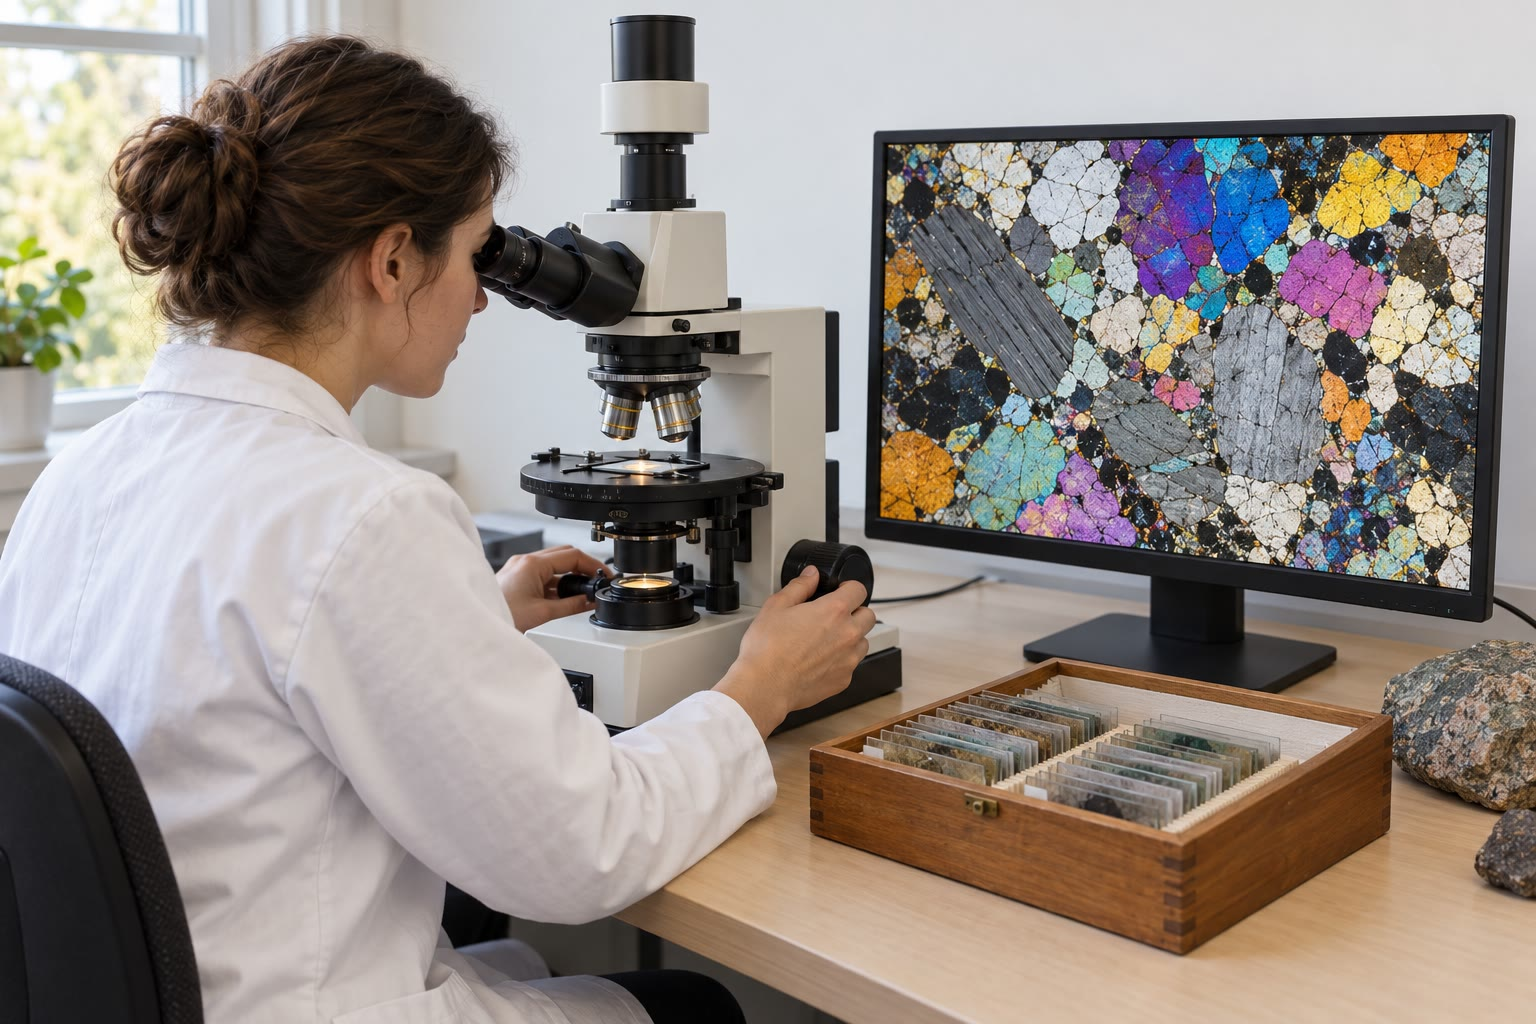
\includegraphics[width=\linewidth]{images/book5/ai/b3-petrology-desk.jpg}

{\scriptsize عالِم صخور عند مجهر مستقطِب، وعلبة من الشرائح الرقيقة
في متناول اليد، وشريحة رقيقة بالضوء المستقطَب على الشاشة
(رسم توضيحي مولَّد بالذكاء الاصطناعي).}
\end{minipage}
\end{inthelab}

\section{التمارين}

\begin{exercise}[$\star$]\label{exo:b3:petrological-thermodynamics:1}
من الجداول، للألبيت $\Delta_fH^\circ = \qty{-3935.0}{kJ}$، و$S^\circ =
\qty{207.4}{J.K^{-1}}$، $V = \qty{100.07}{cm^3}$؛ الجاديت $-3029.3$، 133.5،
60.40؛ الكوارتز $-910.7$، 41.5، 22.69 (لكل مول). بالنسبة إلى التفاعل الألبيت = الجاديت + الكوارتز،
احسب $\Delta_rH$، و$\Delta_rS$، و$\Delta_rV$ (بوحدة \unit{J.bar^{-1}})،
وميلَ كلابيرون، وضغطَ الخطّ عند \qty{600}{\celsius} بافتراض
ثبات الخواصّ.
\end{exercise}
% ledger: rh95:ab-jd-qz

\begin{exercise}[$\star$]\label{exo:b3:petrological-thermodynamics:2}
صخرةٌ من النظام \ce{MgO}--\ce{SiO2} تحتوي على الفورستيريت والإنستاتيت
والكوارتز. طبّق \omterm{prop:b3:petrological-thermodynamics:goldschmidt}{قاعدة الأطوار المعدنية}. ماذا تستنتج؟
\end{exercise}

\begin{exercise}[$\star$]\label{exo:b3:petrological-thermodynamics:3}
احسب النشاطين المثاليين للغروسولار والبيروب في جارنيت ذي
$X_{\text{Ca}} = 0.20$ و$X_{\text{Mg}} = 0.15$، وللأنورثيت في
البلاجيوكلاز ذي $X_{\text{an}} = 0.40$ (موقع واحد).
\end{exercise}

\begin{exercise}[$\star$]\label{exo:b3:petrological-thermodynamics:4}
احسب درجة الحرارة الحرجة لمحلول منتظم ذي $W =
\qty{15}{kJ.mol^{-1}}$. أيّ $W$ يعطي $T_c = \qty{1000}{K}$؟
\end{exercise}

\begin{exercise}[$\star\star$]\label{exo:b3:petrological-thermodynamics:5}
عند \qty{1000}{K}، تعطي الجداول طاقات جيبس للتكوين
$-5432.2$ (الغروسولار)، $-3478.1$ (الأنورثيت)، $-2088.8$ (الكيانيت) و$-730.2$
(الكوارتز)، بوحدة \unit{kJ.mol^{-1}}. احسب $\Delta_rG$ لتفاعل GASP عند
\qty{1}{bar} وضغط توازنه، وقارِنه بالخطّ التجريبي
$P_0 = 22.80\,T - 1093$ (بالبار، \unit{\celsius}).
\end{exercise}
% ledger: rh95:gasp-ht, kn88:gasp

\begin{exercise}[$\star\star$]\label{exo:b3:petrological-thermodynamics:6}
من أجل المحلول المنتظم الوارد في الشكل ($W = \qty{20}{kJ.mol^{-1}}$)، احسب
$G_{\text{خلط}}$ عند $x = 0.5$ و\qty{900}{K}، ثم عند فرع \omterm{def:b3:petrological-thermodynamics:solvus}{منحنى الانحلال} $x =
0.111$. أثبِت أنّ تجزئة بلّورة تركيبها 0.5 إلى الفرعين
تخفض طاقة جيبس لها، وبمقدار كم.
\end{exercise}

\begin{exercise}[$\star\star$]\label{exo:b3:petrological-thermodynamics:7}
كم طورًا يلتقي عند نقطة لا متغيّرة، وكم خطوطًا أحادية التغيّر
تنطلق منها في نظام من ثلاثة مكوّنات؟ وفي حزمة الشكل،
تحقّق من توازن كلٍّ من التفاعلات الأربعة.
\end{exercise}

\begin{exercise}[$\star\star$]\label{exo:b3:petrological-thermodynamics:8}
صخرة ذات تركيب كلي $X_0 = 0.3$ في المحلول المنتظم الوارد في الشكل
بردت إلى \qty{900}{K}، حيث فرعا \omterm{def:b3:petrological-thermodynamics:solvus}{منحنى الانحلال} هما 0.111 و0.889.
احسب نسبة كلّ طور.
\end{exercise}

\begin{exercise}[$\star\star$]\label{exo:b3:petrological-thermodynamics:9}
باستخدام مقياس الضغط \mbox{\textdir TLT GASP $P = P_0 + (3RT/6.21)\ln(X_{\text{Ca}}/X_{\text{an}})$}
(بالبار)، احسب $\partial P/\partial X_{\text{an}}$ عند \qty{900}{K}
و$X_{\text{an}} = 0.30$. بمقدار كم يُحرّك خطأٌ قدره 0.01 في $X_{\text{an}}$
الضغطَ؟
\end{exercise}

\begin{exercise}[$\star\star\star$]\label{exo:b3:petrological-thermodynamics:10}
أثبِت أنّ المنحنى السبيني لمحلول منتظم هو $x(1 - x) = RT/(2W)$. عند أيّ
درجة حرارة تصبح عندها بلّورةُ تركيبها 0.3 غير مستقرّة أمام أيّ
تقلّبٍ صغير، من أجل $W = \qty{20}{kJ.mol^{-1}}$؟ قارِنها بدرجة الحرارة التي
يبلغ عندها \omterm{def:b3:petrological-thermodynamics:solvus}{منحنى الانحلال}، $T = W(1 - 2x)/[R\ln((1 - x)/x)]$، وفسّر
الفرقَ بينهما.
\end{exercise}

\begin{exercise}[$\star\star\star$]\label{exo:b3:petrological-thermodynamics:11}
أثبِت أنّ \omterm{def:b3:petrological-thermodynamics:solvus}{منحنى الانحلال} لمحلول منتظم متناظر يحقّق $RT\ln[x/(1 -
x)] + W(1 - 2x) = 0$، وأنّه يبلغ أقصى قيمة له، $T_c = W/(2R)$، عند $x
= 1/2$.
\end{exercise}

\begin{exercise}[$\star\star\star$]\label{exo:b3:petrological-thermodynamics:12}
تحتوي الصخرة على \qty{2.0}{wt\percent} من \ce{MnO}. لبّ الجارنيت الذي يحتوي على
\qty{10}{wt\percent} من \ce{MnO} يشكّل \qty{8}{wt\percent} من الصخرة، ويُعزل عن المادّة الأساسية.
احسب محتوى \ce{MnO} في \omterm{def:b3:petrological-thermodynamics:pseudosection}{التركيب الكلي
الفعّال}. لماذا يهمّ ذلك للمقطع الزائف لحواف الجارنيت؟
\end{exercise}

\section{مسألة: جارنيت شيست فاردن}

\begin{problem}[{مسألة نهاية الأسبوع --- الضغط ودرجة الحرارة لشيست
متخيَّل، من الجداول وقاعدة الأطوار ونماذج النشاط
وقياس الحرارة والضغط}]
\label{pb:b3:petrological-thermodynamics:1}
% values: calc/ch11.py; gasp_tables.py
صخر الشيست في الأساس الصخري لتلال فاردن، المتحوّل قبل نحو
\qty{480}{Ma}، يحتوي على الجارنيت والبيوتيت والموسكوفيت والبلاجيوكلاز والكيانايت والكوارتز.
عند حافة إحدى حبيبات الجارنيت وفي الحبيبات المحيطة به، يعطي المسبار الدقيق:
الجارنيت $X_{\text{Fe}} = 0.74$، $X_{\text{Mg}} = 0.12$، $X_{\text{Ca}} =
0.10$، $X_{\text{Mn}} = 0.04$؛ البيوتيت $\ce{Mg}/(\ce{Mg} + \ce{Fe}) = 0.45$؛
البلاجيوكلاز $X_{\text{an}} = 0.30$. استخدم جداول هذا الفصل لتفاعل
GASP، ومقياس الحرارة الوارد في مجلد السنة الثانية:
\[
T = \frac{52\,635 + 0.311P}{20.20 - 3R\ln K_D}\quad(T \text{ بالكلفن}, P
\text{ بالبار}),
\]
ومقياس الضغط التجريبي $P = 22.80\,t - 1093 + (3RT/6.21)\ln
(X_{\text{Ca}}/X_{\text{an}})$، حيث $t$ بوحدة \unit{\celsius} و$T$ بالكلفن.
خذ $R = \qty{8.314}{J.mol^{-1}.K^{-1}}$، وكثافة القشرة
\qty{2800}{kg/m^3} و$g = \qty{9.81}{m/s^2}$.

\medskip\noindent\textbf{الجزء الأول --- الجداول.}
\begin{enumerate}
  \item من جدول الملخّص، احسب $\Delta_rH^\circ$، $\Delta_rS^\circ$
        و$\Delta_rV$ لتفاعل GASP.
  \item احسب $\Delta_rG$ عند \qty{298.15}{K} و\qty{1}{bar}. أيُّ الجانبين
        هو المستقرّ عند السطح؟
  \item احسب ضغط الطرف النهائي عند \qty{900}{K} مع ثبات الخواص،
        وميل كلابيرون.
  \item تعطي جداول الحرارة المرتفعة $\Delta_rG = \qty{81.5}{kJ}$ عند
        \qty{900}{K} و\qty{119.8}{kJ} عند \qty{1200}{K} (\qty{1}{bar}).
        احسب الضغطين.
  \item قارِن بالخطّ التجريبي عند درجتي الحرارة نفسيهما.
  \item ما خطأ $\Delta_rH$ الذي يفسّر الفجوة عند \qty{1200}{K}؟
        قارِنه بعدم اليقين المشترك للإنثالبيات الأربع.
  \item لماذا تُغيّر السعات الحرارية النتيجة بهذا القدر الضئيل؟
\end{enumerate}

\medskip\noindent\textbf{الجزء الثاني --- قاعدة الأطوار.}
\begin{enumerate}[resume]
  \item اذكر المكوّنات اللازمة لوصف المعادن الستة ومائع مائي،
        وعُدّ الأطوار.
  \item احسب درجة الحرية بقاعدة الأطوار، وتحقّق من
        \omterm{prop:b3:petrological-thermodynamics:goldschmidt}{قاعدة الأطوار المعدنية}.
  \item تحتوي عيّنة ثانية على الكيانايت والسيليمانيت متجاورَين. ماذا
        تدلّ العيّنة عن ضغطها ودرجة حرارتها؟
  \item تدفّق الماء عبر الصخرة أثناء التحوّل. كيف يغيّر ذلك
        العدّ؟
\end{enumerate}

\medskip\noindent\textbf{الجزء الثالث --- النشاطات وقياس الحرارة والضغط.}
\begin{enumerate}[resume]
  \item احسب النشاطات المثالية للغروسولار والأنورثيت، و$\ln K$
        لتفاعل GASP في الصخرة.
  \item احسب $K_D$ لتبادل الجارنيت--البيوتيت.
  \item احسب درجة الحرارة عند \qty{8}{kbar}.
  \item احسب ضغط GASP عند تلك الدرجة من الحرارة.
  \item كرّر الحساب حتى تبلغ نقطة تقاطع المعادلتين.
  \item أعِد حساب التقاطع بخطّ الطرف النهائي من الجداول بدلًا
        من الخطّ التجريبي (مع $\Delta_rV = \qty{-6.61}{J.bar^{-1}}$).
        أيّ النتيجتين تُعتمد، ولماذا؟
  \item بمقدار كم يُحرّك خطأ قدره 0.05 في $X_{\text{an}}$
        النتيجة؟
\end{enumerate}

\medskip\noindent\textbf{الجزء الرابع --- الطمر.}
\begin{enumerate}[resume]
  \item بالخواص الثابتة الواردة في مجلد السنة الثانية، يكون لتفاعل الكيانايت =
        السيليمانيت $\Delta_rH = \qty{7.7}{kJ}$، $\Delta_rS =
        \qty{12.6}{J.K^{-1}}$، $\Delta_rV = \qty{0.571}{J.bar^{-1}}$. هل
        تقع النتيجة في حقل الكيانايت؟
  \item احسب عمق الطمر.
  \item يحتوي لبّ الجارنيت على $X_{\text{Ca}} = 0.07$ ونما مع البلاجيوكلاز
        بالقيمة $X_{\text{an}}$ نفسها، وعند درجة حرارة متقاربة.
        هل تكوّن اللبّ على عمق أكبر أم أقلّ من الحافة؟
  \item أعطِ ضغط الذروة وعمق الطمر لشيست فاردن.
\end{enumerate}
\end{problem}
